\subsection{Polos y ceros}

Anal\'iticamente se obtienen las siguientes expresiones para los polos y ceros del filtro:

\begin{equation}
s_{z1,z2} = - \frac{R_4  R_6  R_8+R_5  R_6  R_8 - R_4 R_5 R_7}{C_6 R_6 R_7 R_8 \cdot (R_4 + R_5)} \pm \sqrt{\left( \frac{R_4 R_6 R_8 + R_4 R_6 R_8 - R_4 R_5 R_7}{C_6 R_6 R_7 R_8 \cdot (R_4 + R_5)}\right)^2- 4 \cdot \frac{R_4 R_5}{C_2 C_6 R_1 R_3 R_8 \cdot (R_4 + R_5)}}
\label{ceros}
\end{equation}

\begin{equation}
s_{p1,p2} = - \frac{R_6 + R_7}{C_6 R_6 R_7} \pm \sqrt{\left( \frac{R_6 + R_7}{C_6 R_6 R_7}\right)^2 - 4 \cdot \frac{R_4(R_5+R_8)}{C_2 C_6 R_1 R_3 R_5 R_8}}
\label{polos}
\end{equation}


A partir de las expresiones anteriores, al reemplazar con los valores de los componentes empleados, se obtiene el siguiente diagrama de polos y ceros del filtro high pass notch, con $Q\approx 2$:

\begin{figure}[H] %!ht
	\centering
	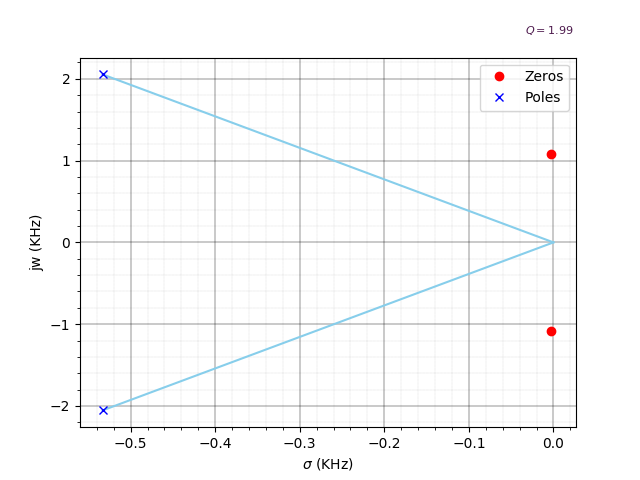
\includegraphics[width=10cm,height=10cm,keepaspectratio]{../EJ1/00GRAFICOS/singularidades.png}
	\caption{Polos y ceros de la funci\'on transferencia del circuito.}
	\label{c1vinmax}
\end{figure}

Los polos se encuentran claramente del lado izquierdo del eje $j\omega$, lo que indica estabilidad del circuito.





